\documentclass[11pt,a4paper]{article}
\usepackage[T1]{fontenc}
\usepackage[utf8]{inputenc}
\usepackage{lmodern,microtype}
\usepackage[margin=.85in]{geometry}
\usepackage{amsmath,amssymb,mathtools}
\usepackage{booktabs,tabularx,array,enumitem,needspace,float}
\usepackage{xcolor,tikz}
\usetikzlibrary{arrows.meta,positioning,fit,calc,backgrounds}
\usepackage[hidelinks]{hyperref}
\usepackage[nameinlink,noabbrev]{cleveref}
\usepackage{fancyhdr}
\hypersetup{pdftitle={Sequencer Rotation Architecture v4},
pdfsubject={Espresso finality, timed control, publication verification, and staking lifecycle}}
\pagestyle{fancy}\fancyhf{}
\lhead{\small Sequencer rotation architecture}\rhead{\small Version 4 / Espresso finality}
\cfoot{\thepage}\setlength{\headheight}{14pt}
\setlength{\parindent}{0pt}\setlength{\parskip}{4pt}
\setlength{\emergencystretch}{2em}
\setlist{nosep,leftmargin=*}
\newcolumntype{Y}{>{\raggedright\arraybackslash}X}
\newcommand{\api}[1]{\ensuremath{\mathsf{#1}}}
\newcommand{\Hash}{\mathsf H}
\newcommand{\RF}{\mathsf{RF}}
\newcommand{\FC}{\mathcal F}
\newcommand{\TB}{\mathit{TB}}
\newcommand{\role}{\textbf{Role and property.}\ }
\newcommand{\iface}{\textbf{Minimal interface.}\ }
\newcommand{\src}[2]{\href{#1}{\texttt{\detokenize{#2}}}}
\definecolor{nearDone}{HTML}{DCEFE2}
\definecolor{nextStep}{HTML}{DFEBFA}
\definecolor{mainFocus}{HTML}{FBE7C6}
\definecolor{interfaceOnly}{HTML}{F0F1F3}

\begin{document}
\begin{center}
{\LARGE Sequencer Rotation Architecture\par}\vspace{5pt}
{\large Version 4: Espresso Finality and Module Interfaces\par}\vspace{8pt}
17 October 2026
\end{center}

\section{Architecture and current priorities}\label{sec:overview}
The system produces a reliable stream of mini-block batches and requires
proposer $P$ to publish exactly a continuous globally final part of that
stream. This version extends
\src{arch_v3.tex}{architecture v3}. Its protocol baseline is
\src{sync_hotstuff_rr_part2_rotation_v3.tex}{Sync HotStuff RR, Part II v3};
\src{sync_hotstuff_rr_part1_core.tex}{Part I} supplies the regional core.
The regional DATA/DRAIN protocol, fixed voting snapshots and regular
handoff remain in place. The full view is now written
$(\beta,r,g,t)$, and a session is $(\beta,r)$. This notation makes
branch separation explicit. The two Force paths and their target check
are unchanged.

Three modules separate transport, external finality and verification.
The \emph{Publisher} sends complete regional results to Espresso.
\emph{Espresso} provides a finalized ordered log with authenticated
timestamps. The \emph{Certifier} checks that log, L1 control and regional
evidence under the same rotation rules as full nodes. Espresso treats
our records as data. It does not run our rotation program or an
application smart contract.

L1 retains the \emph{Staking Service}, \emph{Authority/Schedule},
\emph{Liveness and Force Control}, and \emph{Publication Verifier}.
The multisignature committee writes only to L1. Its status updates and
Forces take effect at announced future Espresso timestamps. Nodes also
derive a block-missing Force when the next export session fails its
fixed delivery window. Both Forces preserve the entire global prefix.
Neither can select an older restart point.

A valid regional result becomes global when its complete, continuous
EXPORT is accepted from finalized Espresso history. There is no
per-block committee protection delay and no wait for that history to
be registered on L1. Regular successors may start from a terminal
regional receipt before this global confirmation. Forced successors
wait for the finalized Espresso boundary and then continue from its
exact global anchor.

\textbf{Design priorities.} Preserve the regional engine and staking
interfaces. Specify the shared rotation interpreter, complete cross-chain
inputs and publication relation. The new service assumptions must be
matched to an Espresso proof and clock profile before implementation.
This document specifies module contracts; it is not an implementation
audit or an unconditional proof of the external services.

\begin{figure}[H]\centering
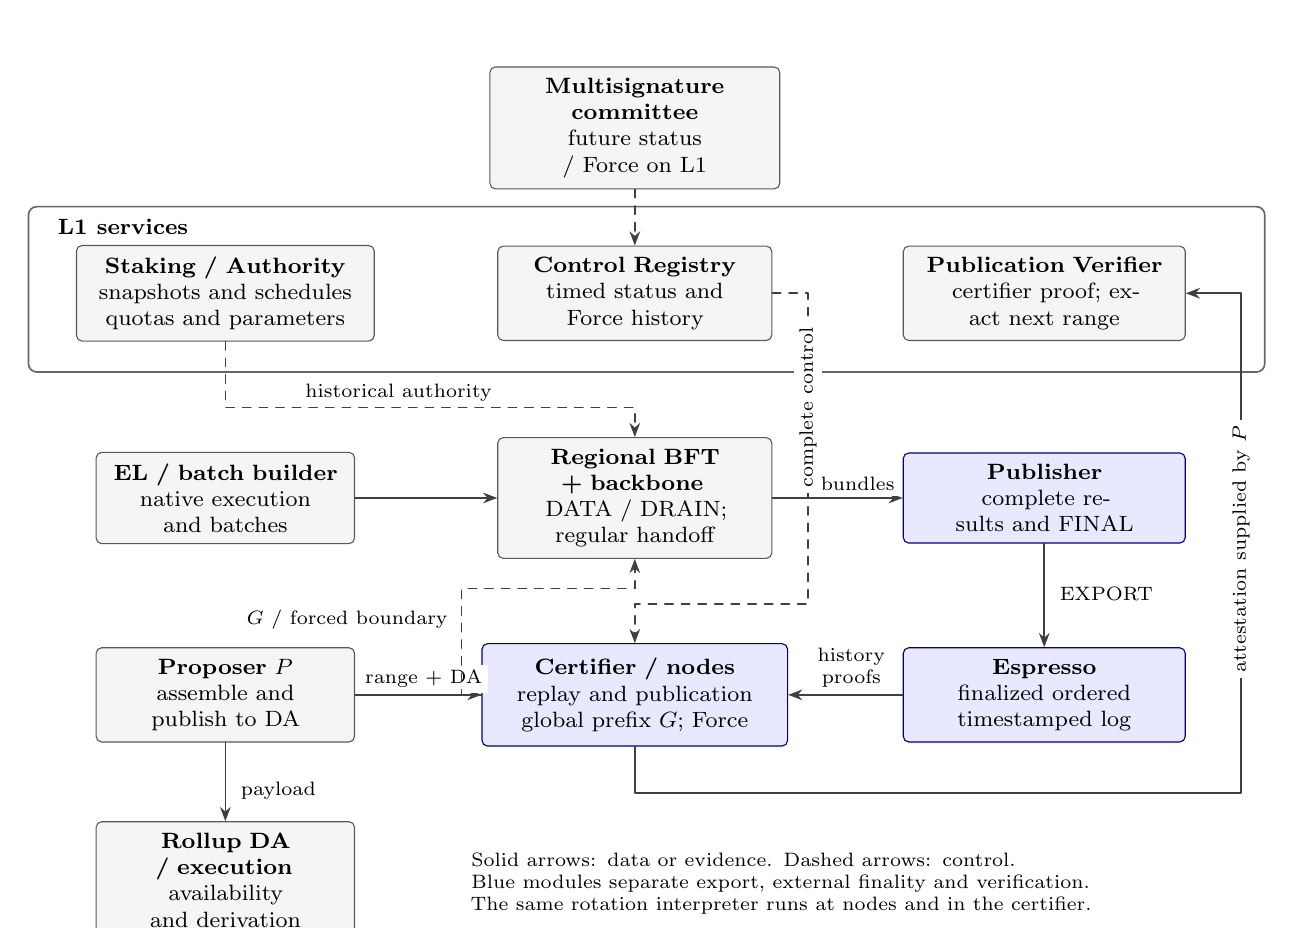
\begin{tikzpicture}[
  x=1cm,y=1cm,font=\footnotesize,line cap=round,line join=round,
  box/.style={draw=black!65,rounded corners=2pt,fill=gray!8,
    align=center,inner sep=4pt,minimum height=1cm},
  new/.style={box,fill=blue!9,draw=blue!50!black},
  flow/.style={-{Stealth[length=1.8mm]},semithick,draw=black!75},
  ctl/.style={flow,dashed},
  lab/.style={fill=white,inner sep=2pt,align=center,font=\scriptsize}
]
  \node[box,text width=3.4cm] (msig) at (7.8,11.1)
    {\textbf{Multisignature committee}\\future status / Force on L1};
  \draw[rounded corners=3pt,semithick,draw=black!60]
    (.1,8.0) rectangle (15.8,10.1);
  \node[anchor=west,font=\footnotesize\bfseries] at (.35,9.85)
    {L1 services};
  \node[box,text width=3.5cm] (stake) at (2.6,9.0)
    {\textbf{Staking / Authority}\\snapshots and schedules\\quotas and parameters};
  \node[box,text width=3.2cm] (control) at (7.8,9.0)
    {\textbf{Control Registry}\\timed status and Force history};
  \node[box,text width=3.3cm] (verify) at (13.0,9.0)
    {\textbf{Publication Verifier}\\certifier proof; exact next range};
  \draw[ctl] (msig.south) -- (control.north);

  \node[box,text width=3.0cm] (builder) at (2.6,6.4)
    {\textbf{EL / batch builder}\\native execution and batches};
  \node[box,text width=3.2cm] (regional) at (7.8,6.4)
    {\textbf{Regional BFT + backbone}\\DATA / DRAIN; regular handoff};
  \node[new,text width=3.3cm] (publisher) at (13.0,6.4)
    {\textbf{Publisher}\\complete results and FINAL};
  \draw[flow] (builder.east) -- (regional.west);
  \draw[flow] (regional.east) -- (publisher.west);
  \node[lab,above] at (10.63,6.42) {bundles};
  \draw[ctl] (stake.south) -- (2.6,7.55) -- (7.8,7.55)
    -- (regional.north);
  \node[lab,above] at (4.8,7.55) {historical authority};

  \node[box,text width=3.0cm] (proposer) at (2.6,3.9)
    {\textbf{Proposer $P$}\\assemble and publish to DA};
  \node[new,text width=3.6cm,minimum height=1.3cm] (cert) at (7.8,3.9)
    {\textbf{Certifier / nodes}\\replay and publication\\global prefix $G$; Force};
  \node[new,text width=3.3cm] (espresso) at (13.0,3.9)
    {\textbf{Espresso}\\finalized ordered timestamped log};
  \draw[flow] (publisher.south) -- (espresso.north);
  \node[lab,anchor=west] at (13.12,5.18) {EXPORT};
  \draw[flow] (espresso.west) -- (cert.east);
  \node[lab,above] at (10.55,3.92) {history\\proofs};
  \draw[flow] (proposer.east) -- (cert.west);
  \node[lab,above] at (5.12,3.92) {range + DA};
  \draw[ctl] (control.east) -- (10.0,9.0) -- (10.0,5.05)
    -- (7.8,5.05) -- (cert.north);
  \node[lab,rotate=90] at (10.0,7.55) {complete control};
  \draw[flow] (cert.south) -- (7.8,2.65) -- (15.5,2.65)
    -- (15.5,9.0) -- (verify.east);
  \node[lab,rotate=90] at (15.5,5.75)
    {attestation supplied by $P$};
  \draw[ctl] (cert.west) -- (5.6,3.9) -- (5.6,5.25)
    -- (7.8,5.25) -- (regional.south);
  \node[lab,anchor=east] at (5.5,4.85) {$G$ / forced boundary};

  \node[box,text width=3.0cm] (da) at (2.6,1.55)
    {\textbf{Rollup DA / execution}\\availability and derivation};
  \draw[flow] (proposer.south) -- (da.north);
  \node[lab,anchor=west] at (2.72,2.68) {payload};
  \node[align=left,anchor=west,text width=9.5cm,font=\scriptsize]
    at (5.6,1.5)
    {Solid arrows: data or evidence. Dashed arrows: control.\\
    Blue modules separate export, external finality and verification.\\
    The same rotation interpreter runs at nodes and in the certifier.};
\end{tikzpicture}
\caption{Architecture v4. The publisher submits regional evidence to
Espresso. Nodes and the certifier interpret its finalized history using
complete L1 control and authority. The proposer supplies the certifier's
attestation and the DA claim to the L1 Publication Verifier. Some data
fetch and historical-authority read paths are omitted.}
\label{fig:architecture}
\end{figure}

\section{Objects and module boundaries}\label{sec:objects}
One consensus DATA block $B_h$ contains one ordered batch $x_h$ of
mini-blocks. DATA height, native mini-block number, EVM block number,
Espresso height and Espresso timestamp are separate indices. DRAIN is
internal consensus bookkeeping and has no application payload.
A session is one region's turn and is identified by $(\beta,r)$.
The full production view is
\[
 (\beta,r,g,t).
\]
Here $\beta$ is the branch version, $r$ is the session index, $g$ is
the recovery generation and $t$ is the leader term. The branch version
starts at zero. A regular handoff keeps $\beta$ and increments $r$.
Each actual Force closes $\beta$ and sets the current version to
$\beta+1$. A stale or repeated control does not increment it. Leader rotation
changes $t$; recovery increases $g$ and restarts $t$ at zero. Each new
session starts at $g=t=0$.
For four numerical examples, see Part II v3,
Section 9.3, ``Four concrete view updates after Force.
They distinguish the latest production turn from the turn that still
owes DATA to the global prefix, and show why a stale MSIG leaves the
view unchanged.

Every signature binds the chain, protocol domain, session $(\beta,r)$,
voting configuration, assigned region and message type. View messages
also bind $(g,t)$ and the L1 authority reference $\api{AUTH}_{r,g}$.
FINAL keeps its session and DATA context without $g$ or $t$, so receipts
can still combine across recoveries. An encoding may hash this context;
the hash is not an additional protocol identity.

\begin{table}[H]\centering\small
\begin{tabularx}{\linewidth}{@{}p{.26\linewidth}Y@{}}
\toprule Shared object & Contract\\\midrule
Snapshot $S_e$ & Immutable regional members, keys and voting weights,
with fixed regional protocol parameters.\\
$\api{AUTH}_{r,g}$ & L1 authority indexed by $(r,g)$.
Generation zero fixes the snapshot and quota; later generations provide
leader schedules only.\\
Branch version $\beta$ & Starts at zero and increments once per actual
Force. Regular handoffs keep the same version.\\
Session $(\beta,r)$ & One region's turn within branch version $\beta$.
Its validated boundary fixes its region, anchor and authority.\\
Regional bundle $\mathcal B$ & DATA, regional FINAL receipts, ancestry,
normal boundary witnesses and historical authority.\\
Selection reference & A finalized Espresso header bound by the terminal
regional DATA; it fixes the starting point for successor selection.\\
EXPORT & Current branch version, expected DATA frontier and digest, complete
consecutive DATA and all evidence needed to accept it.\\
Control record & L1-authorized operation with a control sequence,
history commitment and future Espresso activation timestamp.\\
Forced boundary $\mathcal W$ & AUTO or MSIG cause, triggering Espresso
block, exact retained $G$, successor and authority.\\
Global prefix $G$ & Continuous DATA prefix, its commitment and original
session provenance.\\
Replay checkpoint $S$ & $G$, branch, export duty or pending boundary,
windows, eligibility, control context and Espresso cursor.\\
Publication checkpoint $C_{\rm pub}$ & Last accepted published prefix,
with DATA frontier $a\le h(G)$ and accepted execution state.\\
Publication claim $y$ & Previous checkpoint, exact next interval, native
input commitment, DA commitment and execution-state transition.\\\bottomrule
\end{tabularx}
\caption{Objects shared by the modules. Part II v3 fixes their protocol
semantics; implementation documents fix their encodings.}
\end{table}

\textbf{Three progress frontiers.} The regional branch $R$ can run ahead
through several regular sessions. The global prefix $G$ includes only
results accepted from finalized Espresso records. The publication
checkpoint $C_{\rm pub}$ can lag $G$. The \emph{production session}
produces the newest regional output. The \emph{export session} owes
$G$ its next DATA. Block-missing detection uses the latter.

The trusted genesis checkpoint fixes synthetic anchor evidence and
authenticated L1 and Espresso references. Its pending boundary is
$(i_b,\beta_b,r_b)=(\bot,\bot,-1)$, so it selects session zero by
scanning the full region cycle. The first session is $(\beta,0)$,
normally $(0,0)$; a Force during genesis Waiting can increase $\beta$
before selection. Selection sets $q^{\rm open}_{\beta,0}=q_s$.
The L1 bound $\lambda^{\rm open}_{\beta,0}$ is the maximum of the
genesis L1 reference and the initial authority's publication height. A later trusted checkpoint
retains the corresponding history and bounds.

\textbf{Authority is indexed; evidence is branch-specific.}
L1 need not observe every regular boundary. It publishes
$\api{AUTH}_{r,g}$ by numeric index. A Force-created session that reuses
$r$ reads the same indexed authority for its selected region. The different pair
$(\beta,r)$ separates its votes, locks, receipts and replay state.
The leader $L(\beta,r,g,t)$ is selected for the region assigned to that
session, using $\api{AUTH}_{r,g}$. A Force or a new wall-clock epoch does not replace an
old voting snapshot.

\textbf{Native compatibility.} Preserve the native mini-block encoding.
An outer DATA envelope binds its predecessor, BFT identity, finalized
L1 reference and Espresso selection reference. It commits to exact
native headers, transaction bytes, receipts and boundaries. The pinned
native baseline remains
\src{../megaeth_specs/specs/protocol/blocks.md}{blocks.md} and
\src{../megaeth_specs/specs/protocol/state-sync.md}{state-sync.md}
at \texttt{59797b45}. Native signing authority inside an EVM block is
distinct from the BFT leader. The EL adapter must support a valid
execution and signing continuation at the exact regular or forced anchor.

\textbf{Assumption boundaries.} Part II retains separate regional,
L1, cross-region transport and application-output assumptions. It adds
an explicit Espresso service profile and publication-service conditions.
$T_{\rm L1}$ covers actual control submission through finalized,
complete and verifiable availability to all correct participants,
including certifiers. It already includes propagation and validation.
The model also requires honest future scheduling of controls, complete
control views, Espresso prefix safety and authenticated time. Fixed
export windows need stronger delivery conditions than eventual backbone
transport alone. Certifier integrity and native execution correctness
remain separate assumptions; one does not establish the other.

\section{Staking Service and authority: the main design work}\label{sec:staking}
\subsection{Participation and escrow}
\role Convert public stake-backed applications into immutable voting
snapshots, retain liability for earlier service, and release funds only
after the corresponding obligations end. Permissionless admission uses
public rules; it does not make a pending deposit an immediate voter.

\iface
\[
\begin{aligned}
 &\api{Join}(i,pk,\text{owner},b)\to o,\quad
   \api{Cancel}(o),\quad \api{RequestExit}(o),\\
 &\api{Report}(\text{evidence}),\qquad \api{Claim}(o).
\end{aligned}
\]
Here $o$ is a persistent stake-position identifier, $i$ its registered
region, $pk$ its signing key, and $b$ its bond. The initial profile follows
\src{../formalization/staking_rotation_module_v2.tex}{staking module v2}:
one collateral token, fixed region identifiers and whole-position joins
and exits. Delegation, partial withdrawal and region migration are
extensions. Key possession and withdrawal-owner authorization are checked
at the appropriate calls.

\begin{table}[H]\centering\small
\begin{tabularx}{\linewidth}{@{}p{.22\linewidth}Y@{}}
\toprule Lifecycle stage & Interface meaning\\\midrule
Pending join & Deposit is queued by finalized L1 order. No voting or
leader rights; cancellation is allowed before reservation.\\
Reserved & A frozen plan has selected the position. Its funds cannot be
refunded while activation is pending; the operator prepares to serve.\\
Assigned / active & A finalized authority uses its snapshot. The operator
serves whenever a valid boundary opens the corresponding session.\\
Exit queued & A request to stop receiving future duties. Existing
snapshot votes, participation and data duties remain in effect.\\
Retired / cooling & Retirement clearance establishes that no new valid
duties can arise and existing service obligations have ended. Required
data retention and evidence liability continue.\\
Claimable & Release residual funds after the liability window, retaining
amounts encumbered by timely unresolved claims.\\\bottomrule
\end{tabularx}
\caption{Permissionless entry and exit are a lifecycle, not immediate
edits to an active BFT committee.}
\end{table}

Queues and fixed cutoffs make selection reproducible. Separate inbound
and outbound stake/count budgets bound voluntary churn; canceling a
pending request cannot leave a permanent queue obstruction. Each permitted
whole position must fit its direction's budget. Mandatory removals after
penalties are accounted for separately. Under continued configuration
progress, eligible requests must receive service; an economic preference
for a regional stake floor cannot veto exit forever.

\subsection{Frozen plans and future authorities}\label{sec:authority}
\role Publish a reproducible mapping from stake snapshots to the
authorities consumed by Part II. Authority establishes eligibility;
a REGULAR or forced boundary and Ready establish actual session entry.

\iface
\[
\begin{aligned}
 &\api{Prepare}(e)\to\mathit{Plan}_e,\qquad
   \api{Activate}(\mathit{Plan}_e,\mathcal I_e),\\
 &\api{ReadSnapshot}(e)\to S_e,\qquad
   \api{ReadAuthority}(r,g)\to\api{AUTH}_{r,g}.
\end{aligned}
\]
$\mathcal I_e$ is a finite set or range of future, as-yet-unassigned
session indices. Assigning a range is an architectural option for
amortizing L1 updates, not an extra transaction at each handoff.
\api{Prepare} fixes the selected joins/exits and balances at the public
cutoff. If randomness is used, freeze the plan before obtaining the
prescribed random input and forbid discretionary retries.

\api{Activate} accepts only a frozen, publicly verifiable plan and
establishes an immutable mapping $e(r)$ for the assigned indices, so
the relevant snapshot in $\api{AUTH}_{r,0}$ is $S_{e(r)}$.
An already assigned index cannot be rebound. The snapshot includes
regional members, keys, weights, $F_i$, $\Delta_i$ and $K$; the authority
also fixes $\TB_r$ and the export-window parameters. For $g>0$, only
the new leader schedule is consumed.
The admissible index range and activation condition follow public policy;
the relayer cannot choose them to favor a particular plan or skip queues.
Later finalized schedules can exclude exposed equivocators, while votes
remain measured against the original snapshot. Already finalized
schedules cannot be retroactively rewritten.

The authority service must give members timely access to the rules for
future indices and recovery generations, and must leave actual future
service opportunities for new snapshots. An unbounded advance allocation
of indices to an old snapshot would defeat admission and exit. If a needed
authority is not finalized, Part II waits. A zero-member region must not
be selected under the authority/control combination. Part II's
fixed cyclic region order and \api{NextLive} rule are retained; this
architecture does not import the staking draft's per-epoch region shuffle
or same-region renewal.

\subsection{Retirement clearance and withdrawal}\label{sec:retirement}
\role Connect removal from future stake plans to the end of actual
consensus duties. This is the central unresolved staking interface.
\api{Retired}(o,\text{clearance}) is a lifecycle event produced only after
the service can establish:
\begin{enumerate}
\item future authority assignment will not create new duties for $o$;
\item consensus and signing duties from already assigned indices are
discharged, including
sessions that a valid Force could still open using an old index; and
\item already opened regional engines have reached an allowed stopping
condition, with required history retained or transferred.
\end{enumerate}
The clearance must bind the relevant historical authorities and session pairs
$(\beta,r)$. A new branch version, a region-off status or a Force
activation alone does not establish it. Part II leaves discarded engines running until their
Completion condition; it has no general early-stop rule. This architecture
therefore does not assert a bounded withdrawal time. The staking design must
provide retirement clearance or explicitly retain that dependency.

After clearance, the liability/retention policy sets the release horizon.
Timely accepted unresolved claims retain the affected escrow until
adjudication. Slashing reduces the remaining bond, never the historical
quorum denominator; the same funds cannot be recovered separately for each historical
service assignment. Equivocation evidence binds the old position,
authority and session $(\beta,r)$. Timeout BLAME or a health report is not by
itself slashable equivocation. Historical certificate acceptance and
key-compromise assumptions must match the liability/checkpoint policy.

These interfaces reuse staking v2's queues, reservations and escrow
semantics. They replace its \api{Close}/\api{Advance} coupling: ordinary
Part II handoffs remain off L1, and Force does not close the old regional
engine. Churn and staking alone do not establish $F_i<W_i/2$ in every
serving region.

\section{Multisignature monitor and Liveness/Force Control}\label{sec:force}
\subsection{Off-chain monitoring}
\role Diagnose regional health and submit future eligibility changes or
Forces to L1. Treat the committee as one honest coordinated control
service, with the same scope of trust as the model in Part II. It no
longer protects a prefix by delaying global confirmation. Its internal
membership and diagnosis policy remain outside this architecture.

\iface
\[
 \api{ObserveBundle}(\mathcal B),\quad
 \api{ReportHealth}(i,\text{observations}),\quad
 \api{SubmitControl}(U).
\]
The committee can isolate a region even when that region still delivers
results. It cannot remove global DATA, choose an older anchor, change
historical voting weights or revive a closed branch. A timeout diagnoses
a service failure; it is not by itself evidence of Byzantine conduct.

\subsection{L1 control interface}
\role Authenticate and order control records. Each record binds the
chain, protocol version, sequence number, previous control commitment,
operation and activation timestamp $\theta_a$.

\iface
\[
\begin{aligned}
 &\api{SetStatus}(i,\text{allowed},\theta_a),\qquad
   \api{Force}(\beta,\theta_a,\text{configuration}),\\
 &\api{ReadControl}(\text{checkpoint})\to
   (\text{sequence},\text{history commitment},\text{records}).
\end{aligned}
\]
L1 records authorization. Activation occurs in the shared interpreter,
not when the L1 transaction executes. For an authenticated Espresso
header $J_q$ with timestamp $\theta_q$, define
\[
 \operatorname{cross}(d)=\min\{q:\theta_q\ge d\}.
\]
A control with activation time $d$ acts at the start of
$J_{\operatorname{cross}(d)}$, before its EXPORT payloads. At that
boundary the interpreter applies due status updates, then matching
multisignature Forces, then any block-missing Force, and finally EXPORTs.
Within each control class it orders records by activation time and L1
sequence. Sequence numbers authenticate the complete history; they need
not increase with activation times. Future records stay in a pending
queue until due.

A multisignature Force names the branch version it is intended to stop.
At the activation boundary, the interpreter compares that target with
the branch version at the start of the Espresso block. It applies the
first matching Force in $(\theta_a,c)$ order, where $c$ is the L1
control sequence. It closes that version once and applies no second
Force at the same boundary. Later controls for
the closed version are stale; their attached configuration has no effect.
Independent STATUS or CLEAR records still follow their own rules.
If no matching MSIG Force applies, the interpreter checks AUTO.
A regular regional handoff keeps the same $\beta$, so it does not
cancel a scheduled MSIG Force. At activation, that Force may therefore
close the branch after another region has already taken over.

For example, a scheduled MSIG Force targets version 7. Before it becomes
due, a block-missing AUTO Force closes version 7 and opens version 8.
The later MSIG Force still targets 7, so it does not close version 8 or
apply its attached configuration. This guard prevents two reactions to
the same old failure from forcing the replacement branch again.

Every control must be completely available and finalized before its
activation boundary. $T_{\rm L1}$ already includes that delivery.
If $\theta_q\le t_{\rm E\mbox{-}final}(q)+\epsilon_E$, an honest
committee submitting at real time $s$ can conservatively choose
\[
 \theta_a>s+T_{\rm L1}+\epsilon_E+\text{margin}.
\]
This is a service assumption and scheduling obligation, not a claim
that Ethereum has an unconditional finality bound. Nodes that lack a
complete applicable control view wait. They cannot use local arrival
times to ignore or relocate a late control.

\begin{table}[H]\centering\small
\begin{tabularx}{\linewidth}{@{}p{.24\linewidth}Y@{}}
\toprule Operation & Effect at its Espresso boundary\\\midrule
Ordinary OFF / ON & Changes future selection eligibility. It does not
rewrite an already bound historical selection or revoke old receipts.\\
Matching MSIG Force & Closes the target branch version, preserves $G$,
and applies its authorized configuration atomically.\\
Stale MSIG Force & Does not close a later branch version or apply its conditional
configuration. Independent status records retain their own effect.\\
AUTO Force & Follows a failed export window; closes the branch version and places
the responsible export region in cooldown. No L1 call is required.\\
Cooldown expiry & Restores automatic eligibility at the relevant
Espresso boundary, subject to governance permission and authority.\\\bottomrule
\end{tabularx}
\caption{Control affects future service. It never truncates the global
prefix or silently changes the regional quorum denominator.}
\end{table}

Governance permission, automatic cooldown and authority eligibility are
separate fields. ON does not clear cooldown unless an explicit operation
says so. A ready hint is optional information, not a proof of future
service. Idle regions have no current DATA obligation and are not timed
out for silence. To stop an already opened production branch, the
committee uses Force rather than relying on an ordinary OFF update.

\section{EL, regional BFT and the backbone}\label{sec:sequencing}
\subsection{EL and batch builder}
\role Construct a valid ordered batch and native execution context.
Regional BFT orders this input; the packing policy remains separate.

\iface
\[
 \api{Build}(\text{parent context},\text{requests})\to x,\qquad
 \api{ValidBatch}(x;\text{parent context}).
\]
Validation binds exact bytes, order, multiplicity, mini-block boundaries,
native positions and permitted block context. Receipts and gas fields
must match execution. Global acceptance requires the stated application
output contract. Discovering invalid committed input only at publication
can stop the publication stream, since $P$ may not skip global DATA.

The native adapter owns EVM-boundary assembly and signing-key continuity
across leader and region changes. A valid empty DATA payload consumes
quota and counts under the fixed export-window policy without creating
a native EVM block. That progress metric does not prove resistance to
censorship. Requests remain pending until global inclusion. Requests in
a discarded regional suffix return to consideration under Part II's
admission and queue rules.

A forced anchor may end inside an EVM block. The adapter must support
that exact continuation, or the agreed export profile must make every
possible global endpoint recoverable. A Force cannot round $G$ down to
an earlier EVM boundary. Neither Espresso finality nor certifier
attestation creates a missing native signing key.

\subsection{Regional BFT and cross-region composition}
\role Provide fixed-snapshot SMR, regular leader rotation, recovery and
regional commit evidence. The cross-region handler composes these
engines through certified boundaries.

\iface
\[
\begin{aligned}
 &\api{Open}((\beta,r),\mathcal W,\api{AUTH}_{r,0}),\quad
   \api{Propose}(x),\quad \api{RegionalOutput}(B,\pi_R),\\
 &\api{Boundary}(\mathcal W),\qquad
   \api{BranchChanged}(G,\mathcal W).
\end{aligned}
\]
A regional receipt $\pi_R$ contains FINAL weight $>F_i$ under its fixed
snapshot, where $F_i<W_i/2$. A same-session receipt may cover DATA
ancestors through verified ancestry. A later session's receipt cannot
replace the earlier session's evidence. Proposal QC is not FINAL.
External verification also checks that rotation assigned the DATA to
this session and region.

The DATA/DRAIN structure is unchanged. Normal leader rotation uses a
terminal QC below the session endpoint
$H_{\beta,r}=h(A_{\beta,r,0,0})+\TB_r$ and preserves commit timers. Recovery changes
generation, waits for its authority and preserves the snapshot and
quota. Recovery-only DRAIN can complete the terminal DATA commitment.
DRAIN carries no application batch, copies $T_{\beta,r}$'s L1 and Espresso
references, and does not count toward global DATA progress. Completion
stops a replica's production, voting and
unfinished timers only after it holds the terminal regional receipt;
data service continues.

A regular witness inherits terminal DATA $T_{\beta,r}$ and its regional receipt.
The signed envelope binds a finalized Espresso selection reference
$\xi(T_{\beta,r})=(q,\Hash(J_q))$, whose timestamp is $\vartheta(T_{\beta,r})=\theta_q$.
Its authenticated history determines the first eligible other region
under $\api{AUTH}_{r+1,0}$. If there is no candidate at that reference,
selection waits for the first later authenticated eligible position.
References are nondecreasing and obey the session's lower bound. Each
selection reference must strictly precede the Espresso block containing
its EXPORT. Its historical eligibility snapshot must be authenticated.
Once selected, a witness is not recomputed from the latest status map.
The selected height $q_s$ sets $q^{\rm open}_{\rm next}=q_s$. The
separate L1 lower bound $\lambda^{\rm open}_{\rm next}$ is the maximum
of the anchor's L1 reference height and the L1 height that published
the next initial authority.
Each successor member enters at its own Ready event after checking the
witness, complete state and authority. The session $(\beta,r+1)$ is known before
future EXPORT inclusion.

Normal handoff waits for neither global confirmation nor publication
verification nor a new L1 transaction. Its historical selection rule
may use an older health view; Force is the mechanism for closing that
whole branch. Both Force types retain the exact $G$ before the triggering
Espresso block's payload, close all future appends from the old branch version,
and select a successor using the effective eligibility. With an assigned
export duty, the cyclic search starts after its captured region and the
next numerical session index is its index plus one. It may reuse an
index from a discarded speculative successor, while the pair
$(\beta+1,r_{\rm next})$ keeps protocol state separate.

Every pending handoff stores its source region $i_b$ and predecessor
session $(\beta_b,r_b)$; its next index is $r_b+1$. A regular terminal boundary stores the completed session's
region and session pair. A Force during Waiting reuses
that context; it does not increment a session that never opened. It
replaces the pending boundary, increments $\beta$, retains $G$, and restarts the
selection search from the triggering Espresso height.

A forced successor starts only after it verifies the finalized trigger,
complete control context, exact anchor and required state. Its output
cannot be accepted in the same Espresso block that opened its branch version.
If no other eligible region exists, the protocol waits. Force changes
the external branch, not the old engine's commitment state or stopping
rule. An earlier stopping rule would require a separate protocol change.

\subsection{Backbone and data retention}
\role Carry complete batches, FINAL receipts and witnesses between
regions, publishers, the committee and $P$. Keep retained anchors
recoverable after a region fails.

\iface
\[
 \api{Publish}(\mathcal B),\qquad
 \api{Fetch}(\text{range or object}),\qquad
 \api{Relay}(\mathcal B).
\]
Ordinary backbone delivery remains eventual. Export liveness separately
requires a complete regional result to reach a working publisher and
Espresso within the configured service window. Backup publishing needs
payloads and enough FINAL messages, not just knowledge that a receipt
exists elsewhere. Correct replicas broadcast FINAL and relay complete
receipts and their dependencies. Native state-sync streams may supplement
the evidence path. Transport does not grant finality or replace rollup
DA. Data duties survive Completion and Force until recovery, publication
and retirement obligations are discharged.

\section{Publisher: regional results to Espresso}\label{sec:publisher}
\role Deliver complete regional results and track whether they enter
$G$. The publisher has no content authority. A region may operate a
primary worker, but replicas, successor regions and external services
may submit the same valid result without its permission.

\iface
\[
\begin{aligned}
 &\api{Receive}(\mathcal B),\quad
   \api{FetchMissing}(\text{anchor},\text{target}),\\
 &\api{BuildExport}(G,\text{range},\text{evidence})\to X,\quad
   \api{Submit}(X),\quad \api{Track}(\text{output ID}).
\end{aligned}
\]
An EXPORT $X$ binds the chain, protocol version, branch version, expected
DATA frontier and digest, ordered consecutive DATA, regional receipts, normal
boundary witnesses, historical authority and native context. It may
cross several regular sessions if it includes each session's evidence.
It cannot skip the current export session's missing output. The expected
base binds the DATA prefix, not changing replay fields such as the
Espresso cursor or window counters.

The interpreter checks the complete package before accepting it
atomically. Acceptance appends exactly its stated continuous interval.
Malformed, stale-base or wrong-branch records do not change $G$ or reset
windows. Missing authenticated source data makes verification wait;
it is not evidence that the namespace was empty. A record that failed
at its original position is not inserted there later. A publisher must
fill the gap and resubmit a valid package at a new position.

An output ID binds DATA content and provenance, not a particular set of
signers or encoding. Duplicate receipts do not produce more DATA
progress. Submit-API success and raw inclusion are not acceptance into
$G$. Workers track the accepted prefix and rebuild packages after a
competing publisher or a Force advances the state.

First-submission policy, service fees and publisher replacement are
separate operating choices. A backup service must actually obtain data,
have inclusion access and pay its costs. A reward alone is not a liveness
assumption. Block-missing recovery does not automatically justify
slashing the proposer, current leader or primary publisher.

\section{Espresso: finalized log and common time}\label{sec:espresso}
\role Provide a prefix-consistent finalized log and authenticated
record positions and timestamps. Espresso orders the namespace bytes;
it does not interpret regional authority, quotas, statuses, Force or
native execution.

\iface
\[
\begin{aligned}
 &\api{SubmitNamespace}(X),\qquad
   \api{FetchFinalized}(q_0,q_1),\\
 &\api{VerifyHistory}(\text{trusted anchor},\text{proofs})
   \to (J_{q_0},\ldots,J_{q_1},\text{complete namespace}).
\end{aligned}
\]
The chosen service profile must fix finality evidence, quorum changes,
namespace completeness or authenticated absence, data availability,
retention and timestamp semantics. Headers have nondecreasing timestamps;
height and within-block position give the actual total order. Equal
timestamps do not merge blocks or reopen an earlier deadline.

Future control scheduling requires the chosen clock lead bound or an
equivalent direct advance-availability assumption. Timers also require
timestamps to keep advancing under normal service. An API timestamp
field alone does not establish these properties. Implementation must
pin the Espresso version and proof profile that supply them.

Neither AUTO nor MSIG Force needs an Espresso smart contract or a system
transaction. They are deterministic consequences of complete finalized
inputs. A derived event can be stored for audit, but it is evidence of
the same transition, not a second authorization. Espresso outage stops
new global confirmation. Its recovery can cause a missed delivery
window; that event does not identify which component was at fault.

\section{Certifier and Publication Verifier}\label{sec:publication}
\role The certifier replays the same rotation rules as full nodes and
binds the exact next global interval to a DA publication. The L1
Publication Verifier checks its proof or attestation and the publication
relation. The certifier adds no voting round and cannot choose a
preferred branch independently of the authenticated history.

\subsection{State and interface}
The replay checkpoint $S$ stores $G$, branch version, export session,
quota progress, window state, governance history, cooldowns, complete
control context, pending controls, pending-boundary context, and the
Espresso cursor and trust anchor. It is separate from $C_{\rm pub}$ and its execution state
$z_{\rm pub}$. L1's stored global checkpoint can lag the global prefix
already verified by nodes.

\iface
\[
\begin{aligned}
 &\api{VerifyAndReplay}(S_0,\text{Espresso interval},
       \text{L1 context},\text{regional evidence})\to S_1,\\
 &\api{BindPublication}(C_{\rm pub},S_1,y,\pi)
       \to(C_{\rm next},\text{attestation}),\\
 &\api{VerifyAndAccept}(y,\text{attestation})\to C_{\rm next}.
\end{aligned}
\]
The first two calls run in the certifier; the last runs on L1.
A host fetches evidence, but it cannot declare a source complete,
a block global or a deadline expired. The verified core checks inputs
against its trusted checkpoints. It uses no host-supplied observation
time to decide a global boundary.

The Espresso verification, cursor, TEE registration and DA-binding
structure in
\href{https://github.com/megaeth-labs/specification/blob/aedc2826663b134ee25d26bea17e70c6d23d321c/specs/block-certification/certifier.md}{specification PR \#8, certifier draft}
is a reuse point. Regional receipts, timed L1 control, export windows and
cross-region replay are new checks. The draft is not an unchanged
implementation of this architecture.

\subsection{Shared global-finality tracking}\label{sec:tracker}
For each complete finalized Espresso block, the interpreter first applies
all due control and automatic events. It then processes EXPORTs in
namespace order. A complete EXPORT extends $G$ only if its branch is
open, its expected DATA base matches $G$, its DATA are consecutive and its
regional evidence, native context, authority and session boundaries
are valid. Every accepted DATA is immediately global at that position.
There is no old observation timer or committee-protection wait.

Block-missing checks follow the \emph{export session}, even if regional
production has already handed off several times. When export duty opens
at timestamp $\theta_0$, the startup window is
\[
 [\theta_0,\theta_0+W_{\rm start}),\qquad
 m=\min(m_{\rm start},\text{remaining quota}).
\]
Later fixed windows have length $W_{\rm run}$ and target
$\min(q_{\min},\text{remaining quota at window opening})$.
Authority fixes these positive parameters, the quota and cooldown length
$C_{\rm auto}$ for that session. Only new DATA accepted into $G$ counts;
QC, DRAIN, duplicates and heartbeat do not. Extra DATA in one window
does not prepay later windows.

At the first block crossing a deadline, the interpreter checks the old
window before its payload. A successful window advances to the next
fixed interval. A failed window causes AUTO Force. If a timestamp jump
crosses several deadlines, it settles them in order until the first
failure. An immediate forced successor receives a fresh startup budget
at the trigger timestamp. After Waiting, the budget starts at the first
eligible canonical selection position. It is never backdated to a past
deadline. Completing quota cancels the old windows and moves export duty
to the regular successor. A proven lack of candidates enters Waiting
with no assigned duty or timer. Missing evidence instead pauses replay
at its canonical position. Fetching that evidence later does not create
a later opening time.

Both Force types execute one closing function: retain current $G$,
close all later appends from the old $\beta$, cancel its windows and
choose a successor under the defined current eligibility context.
Each actual Force increments $\beta$ once and records the cause,
finalized trigger and retained anchor. A new version can wait before
opening its next session. That session is $(\beta,r_{\rm next})$;
its witness fixes the successor, authority and selection position. A matching MSIG Force takes priority over an old AUTO check
at the same block; stale or repeated controls do not create another
boundary. Ordinary status updates do not invalidate already bound
historical regular witnesses.

This rule gives all correct replayers the same prefix under the stated
input and service assumptions. It does not tolerate an omitted control
being applied retroactively after $G$ has advanced. Such a discovery
violates the assumed complete control service; it is not a permitted
rollback or a rule to ignore late messages locally.

\subsection{Cross-chain evidence and attestation}
The certifier verifies all of the following:
\begin{enumerate}
\item finalized L1 authority and the complete required control history,
including its sequence, commitment and pending future operations;
\item Espresso finality, validator/quorum provenance, ordered headers
and complete namespace contents or authenticated absence;
\item deterministic status activation, both Force rules, successor
selection and all regional evidence for the exact DATA interval; and
\item correspondence between that interval, native inputs, DA bytes and
the applicable execution-verification result.
\end{enumerate}
An inclusion proof for one favorable event does not prove that no other
control or namespace record occurred. An old but valid L1 checkpoint
is not automatically complete enough for a later Espresso interval.
Online nodes rely on the defined $T_{\rm L1}$ service; new or offline
nodes synchronize before announcing more global DATA.

The attestation binds the chain, protocol version, destination contract,
previous and next replay checkpoints $S_0,S_1$, publication checkpoints,
Espresso interval and trust provenance,
L1 control sequence and commitment, derived rotation state, exact DATA
range, native input commitment, DA evidence and execution result. A TEE
profile must also bind the approved program and registered key. Program
upgrades, key revocation and trusted-checkpoint changes have their own
governance and security assumptions. Daily liveness control does not
include arbitrary permission to change them.

An initial L1 acceptance policy can require the attested control
commitment to match the registry's required current commitment.
If it changed, the certifier refreshes its evidence and attestation.
A refined policy may prove that the control prefix covers all operations
applicable to the processed interval. Either policy must reject omitted
applicable controls. Waiting for refreshed publication evidence affects
$C_{\rm pub}$, not the already established $G$.

The forced successor verifies Espresso and L1 evidence directly.
It does not wait for Espresso's public Ethereum light client to store
the anchor, or for the L1 Publication Verifier to catch up. L1 acceptance,
settlement and withdrawal finality remain later stages.

\subsection{Publication acceptance}
Let $a$ be the accepted publication frontier. A claim is
\[
 y=(C_{\rm prev},[a+1,b],C_{\rm in},C_{\rm DA},z_{\rm pre},z_{\rm post}).
\]
The structured input commitment $C_{\rm in}$ binds exact native headers,
transaction order and multiplicity, mini-block boundaries and execution
context. The L1 verifier accepts only if:
\begin{enumerate}
\item $C_{\rm prev}=C_{\rm pub}$ and $z_{\rm pre}=z_{\rm pub}$;
\item the authenticated certifier result binds $C_{\rm in}$ to the
complete next interval $[a+1,b]$ of $G$, with no omissions, insertions,
reordering or replay;
\item decoding the data committed by $C_{\rm DA}$ gives that same input,
and the selected DA availability and retention predicates hold; and
\item execution verification confirms the transition from $z_{\rm pre}$
to $z_{\rm post}$, including receipts, gas and native assembly.
\end{enumerate}
A height comparison or proof of several individual global leaves is
not enough. The exact next interval is required. A successful update
advances $C_{\rm pub}$ to height $b$ and records $z_{\rm post}$.
It does not create global finality for an unconfirmed input.

Native system transactions are committed or deterministically derived
by the adapter. $P$ cannot add discretionary user transactions. A pending
or disputed execution claim does not advance the accepted publication
frontier. The endpoint must support its native checkpoint or an explicit
partial-EVM continuation. Execution verification may use direct checks,
a validity proof or a sound dispute procedure under its own interface.

Espresso availability does not replace rollup DA. A fallback derivation
rule that discards ordinary content after it entered $G$ is incompatible
with this architecture's global-prefix promise. Any reuse of the PR
\#8 derivation paths must preserve the accepted input prefix or revise
that promise explicitly. Publication delay or a Force cannot erase
old global backlog.

\section{Proposer \texorpdfstring{$P$}{P}}\label{sec:proposer}
\role Fetch global batches, prepare native execution and DA data, obtain
certifier evidence and submit the next complete publication interval.
$P$ may prepare from regional output speculatively. Final acceptance
requires a verified global interval and every publication check above.

\iface $P$ supplies $y$ and its evidence to the certifier, publishes the
matching DA bytes and calls \api{VerifyAndAccept} with the attestation.
An operator may run both $P$ and a publisher, but their interfaces are
different: the publisher exports to Espresso; $P$ publishes the exact
accepted range to rollup DA and L1.

After a Force, retained backlog from old sessions still precedes new
input. Proposer replacement resumes from $C_{\rm pub}$, which may lag
both production and global confirmation. $P$ has no privileged power
to declare input global. Faithful acceptance is a safety property even
for Byzantine $P$. Eventual publication also needs an available proposer
or replacement path, native execution/signing, certifier service and DA.
The verifier cannot make an absent service deliver.

\clearpage
\section{Module index and next design steps}\label{sec:index}
\begin{table}[H]\centering\small
\begin{tabularx}{\linewidth}{@{}p{.22\linewidth}Y Y@{}}
\toprule Module & Primary contract & Next deliverable\\\midrule
Regional BFT & Part I and Part II v3; \cref{sec:sequencing}
& Preserve DATA/DRAIN, FINAL, Completion and Ready; bind the new history
references and identities.\\
Staking / authority & \cref{sec:staking,sec:authority,sec:retirement}
& Freeze future snapshots, fix window parameters and complete retirement
clearance and withdrawal liability.\\
Monitor / L1 control & Part II v3 time model; \cref{sec:force}
& Future timestamp scheduling, complete control history and explicit
eligibility permissions.\\
Publisher & \cref{sec:publisher}
& Complete-bundle retrieval, backup submission, acceptance tracking and
retention.\\
Espresso & \cref{sec:espresso}
& Pin finality, namespace, quorum, availability and timestamp profiles.\\
Certifier / L1 verifier & \cref{sec:publication}
& Shared replay, complete cross-chain context, attestation binding and
exact range/DA verification.\\
EL / backbone / proposer & \cref{sec:sequencing,sec:proposer}
& Recover exact native state, retain data and publish every next interval.\\\bottomrule
\end{tabularx}
\caption{Module boundaries and remaining integration work.}
\end{table}

The integration order is to retain the regional engine, implement one
shared interpreter, connect complete L1 and Espresso evidence, and bind
its accepted prefix to faithful publication. Window values require an
explicit end-to-end delivery budget that covers regional recovery,
backup publishing, Espresso inclusion and state retrieval. Eventual
transport alone does not justify fixed-time progress. With no eligible
other region, the baseline waits; same-region renewal is a separate
extension.

Staking remains a distinct lifecycle problem. Force does not close old
regional engines or discharge their data duties, so it does not prove
retirement clearance. The new finality service changes the global
confirmation rule, not the regional Byzantine bound or the authority
of historical signatures. These boundaries should remain explicit in
implementation and subsequent proofs.
\end{document}
